%--------------------------------------------------------------------
% NE 155 (intro to numerical simulation of radiation transport)
% Spring 2017

% formatting
\documentclass[12pt]{article}
\usepackage[top=1in, bottom=1in, left=1in, right=1in]{geometry}

\usepackage{setspace, multicol}
\onehalfspacing

\setlength{\parindent}{0mm} \setlength{\parskip}{1em}


% packages
\usepackage{amssymb}
%% The amsthm package provides extended theorem environments
\usepackage{amsthm}
\usepackage{epsfig}
\usepackage{times}
\renewcommand{\ttdefault}{cmtt}
\usepackage{amsmath}
\usepackage{graphicx} % for graphics files

% Draw figures yourself
\usepackage{tikz} 

% The float package HAS to load before hyperref
\usepackage{float} % for psuedocode formatting
\usepackage{xspace}

% from Denovo methods manual
\usepackage{mathrsfs}
\usepackage[mathcal]{euscript}
\usepackage{color}
\usepackage{array}

\usepackage[pdftex]{hyperref}

\newcommand{\nth}{n\ensuremath{^{\text{th}}} }
\newcommand{\ve}[1]{\ensuremath{\mathbf{#1}}}
\newcommand{\macro}{\ensuremath{\Sigma}}
\newcommand{\vOmega}{\ensuremath{\hat{\Omega}}}

\newcommand{\Macro}{\ensuremath{\Sigma}}


\newcommand{\cc}[1]{\ensuremath{\overline{#1}}}
\newcommand{\ccm}[1]{\ensuremath{\overline{\mathbf{#1}}}}


%--------------------------------------------------------------------
%--------------------------------------------------------------------
\begin{document}
% Iterative methods
The \textbf{fixed-point} iterative process and associated error are (where $\rho(\ve{P})$ is the spectral radius of $\ve{P}$.):
\[\vec{x}^{(0)} = \text{ arbitrary}\:; \qquad
\vec{x}^{(k+1)} = \ve{P}\vec{x}^{(k)} + \tilde{\vec{b}} \]
\[\vec{e}^{(k+1)} = \ve{P}\vec{e}^{(k)}\:; 
 \qquad ||\vec{e}^{(k+1)}|| \leq ||\ve{P}^{k+1}||\: ||\vec{e}^{(0)}||\:;
 \qquad || \ve{P}^k || \approx \rho^k (\ve{P})\]
%
To reduce error by a factor of $\epsilon$, it takes $k \approx \frac{\log(\epsilon)}{\log(\rho(\ve{P}))}$ iterations. 
%
    \begin{table}[h!]
    \centering
      \begin{tabular}{| c | c | }
        \hline
        Richardson & Jacobi \\ \hline
        \hline
        $(\ve{I} - \omega^{(k)}\ve{A})\vec{x}^{(k)} + \omega^{(k)}\vec{b}$   &  
        $ \ve{D}^{-1}(\ve{D} - \ve{A})\vec{x}^{(k)} + \ve{D}^{-1}\vec{b}$  \\
        \hline  
        GS & SOR \\ \hline
        $ (\ve{D} + \ve{L})^{-1} \bigl[-\ve{U} \vec{x}^{(k)} + \vec{b}\bigr] $ &  
        $ (\ve{D} + \omega \ve{L})^{-1} \Bigl( [(1-\omega)\ve{D} - \omega \ve{U}] \vec{x}^{(k)} + \omega\vec{b} \Bigr)$ \\
        \hline        
      \end{tabular}
      \caption{$\vec{x}^{(k+1)}$ for several iterative methods}
      \label{tab:delayedneutrons}
    \end{table}
%\begin{align*}
%\text{Richardson} \qquad &\vec{x}^{(k+1)} = (\ve{I} - \omega^{(k)}\ve{A})\vec{x}^{(k)} + \omega^{(k)}\vec{b}\:;
% \qquad x^{(k+1)}_i =  x^{(k)}_i - \omega^{(k)} \sum_{j=1}^{n} a_{ij}x_j^{(k)} + \omega^{(k)} b_i \\
%%
%\text{Jacobi} \qquad & \vec{x}^{(k+1)} = \ve{D}^{-1}(\ve{D} - \ve{A})\vec{x}^{(k)} + \ve{D}^{-1}\vec{b}\:;
%  \qquad x^{(k+1)}_i = \frac{1}{a_{ii}}(b_i - \sum_{j=1}^{i-1} a_{ij} x_j^{(k)} - \sum_{j=i+1}^{n} a_{ij} x_j^{(k)})\\
%%
%\text{GS} \qquad &  x^{(k+1)}_i = \frac{1}{a_{ii}}(b_i - \sum_{j=1}^{i-1} a_{ij} x_j^{(k+1)} - \sum_{j=i+1}^{n} a_{ij} x_j^{(k)})\\
%%
%\text{SOR} \qquad & x^{(k+1)}_i = (1-\omega)x_i^{(k)} + \frac{\omega}{a_{ii}}(b_i - \sum_{j=1}^{i-1} a_{ij} x_j^{(k+1)} - \sum_{j=i+1}^{n} a_{ij} x_j^{(k)}) 
%\end{align*}
%

\vspace*{-1em}
\textbf{condition number} of a matrix $\mathbf{A}$ is defined as $\kappa(\mathbf{A}) = ||\mathbf{A}|| \text{ }||\mathbf{A}^{-1}||$.
%
If the 2-norm is used, then $||\mathbf{A}||_{2} = \sigma_{1}$, $||\mathbf{A}^{-1}||_{2} = 1 / \sigma_{m}$, and $\kappa_{2}(\mathbf{A}) = \sigma_{1} / \sigma_{m}$; $\sigma_{m}$ is the $m$th singular value of $\ve{A}$. %If $\mathbf{A}$ is singular, its condition number is infinity. 

Let $\ve{G}$ be a non-singular \textbf{preconditioner}, then $\ve{A}\vec{x}=\vec{b}$ can be transformed as $\ve{G}^{-1}\ve{A}x = \ve{G}^{-1}b$.

% finite difference
\textbf{Finite Difference} for the DE in \underline{1D} we use central difference for the derivative: 
\[-\phi_{i-1} + \bigl(2 + \frac{h^2}{L^2}\bigr)\phi_i - \phi_{i+1} = h^2 \frac{S_{0,i}}{D} \qquad i = 1, 2, \dots, n-1\]

In \underline{2D} we use a 5-point stencil and use central in each dimension for the derivative, giving
\[ \nabla^2 \phi_{i,j} = \frac{\phi_{i+1,j} + \phi_{i-1,j} + \phi_{i,j+1} + \phi_{i,j-1} - 4\phi_{i,j}}{h^2}\]


% finite volume
\textbf{Finite Volume} for the DE in \underline{1D} uses this grid 
%
\begin{multicols}{2}
\begin{center}
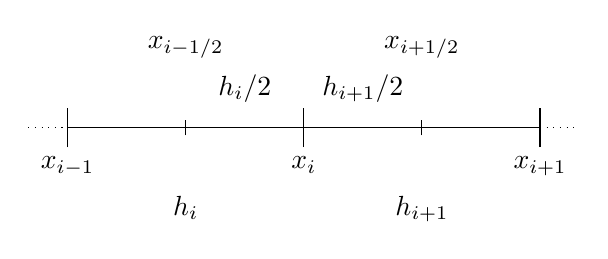
\begin{tikzpicture}
\draw[dotted] (0,0)--(0.5,0);
\draw (0.5,0)--(3.5,0);
\draw (.5,-.25)--(.5,.25);
\draw (2,-.1)--(2,.1);
\draw (3.5,-.25)--(3.5,.25);
\draw (0.5,0)--(6.5,0);
\draw[dotted] (6.5,0)--(7,0);
\draw (.5,-.25)--(.5,.25);
\draw (5,-.1)--(5,.1);
\draw (6.5,-.25)--(6.5,.25);
\node[below] at (.5,-.25) {$x_{i-1}$};
\node[below] at (6.5,-.25) {$x_{i+1}$};
\node[below] at (3.5,-.25) {$x_i$};
\node[above] at (2, 0.75) {$x_{i-1/2}$};
\node[above] at (5, 0.75) {$x_{i+1/2}$};
\node[below] at (2, -.75) {$h_{i}$};
\node[below] at (5, -.75) {$h_{i+1}$};
\node[above] at (4.25, .2) {$h_{i+1}/2$};
\node[above] at (2.75, .2) {$h_{i}/2$};
\end{tikzpicture}
\end{center}
\columnbreak
The physics values are defined in each cell (cell-centered) and the flux and source are defined at the mesh points (edge-centered.\\
We integrate the DE in each cell from $x_{i-1/2}$ to $x_{i+1/2}$. At the boundaries we apply the BCs as appropriate to get the $i=0$ and $i=n$ equations.
\end{multicols}


The \underline{2D} version uses a 2D stencil (not needed for exam). The physics values are again defined in each cell (cell-centered) and the flux and source are defined at the mesh points (edge-centered.\\
We again integrate over the partial cell, which is now in two dimensions: $x_{i-1/2}$ to $x_{i+1/2}$ and $y_{j-1/2}$ to $y_{j+1/2}$.\\
We use Gauss Theorem for the streaming term: $-\int_V d\vec{r}\:\bigl[\nabla \cdot \bigl(D(\vec{r})\nabla \phi(\vec{r})\bigr)\bigr] = \int_S d\vec{S} \:D(\vec{r})\frac{\partial}{\partial \hat{n}}\phi(\vec{r})$.


\end{document}